\subsection{Performance Portability Visualization}
\label{sec:pp_visualization}

\citet{sewall_interpreting_2020} 
different visualization strategies:
\begin{itemize}
    \item Box Plots: obscures the "did not run" case (large boxes); no number of supported platforms; only median to compare in case of "did not run" (boxes cover whole range)
    \item Histograms: distribution of bins ("did not run" must be own bin; how many bins?); areas of low density $\rightarrow$ difficult to "see" the distribution
    \item Probability Density Function: primary problem choosing a good kernel bandwidth; PP sparse and uneven distributed data $\rightarrow$ no fixed bandwidth guaranteed to yield satisfactory results $\rightarrow$ adaptive methods; problems on [0, 1] boundaries $\rightarrow$ there may be many points there for PP making this problem even worse; but better than Histograms (better tendencies; less crowded bars)
    \item Violin Plots: a combination of kernel density estimation and Box Plots

    % Impact of Platform Selection
    \item plotting \pp against $\mathcal{H}$ $\rightarrow$ other paper \cite{deakin_performance_2019}
    \item Efficiency Cascade Plots + Platform Charts: minimum efficiency and H $\rightarrow$ remove platform with minimum efficiency and start again; independent for each application; platform sets at the bottom may not be the same for each application; monotonic decreasing
\end{itemize}

\begin{figure}
    \centering
    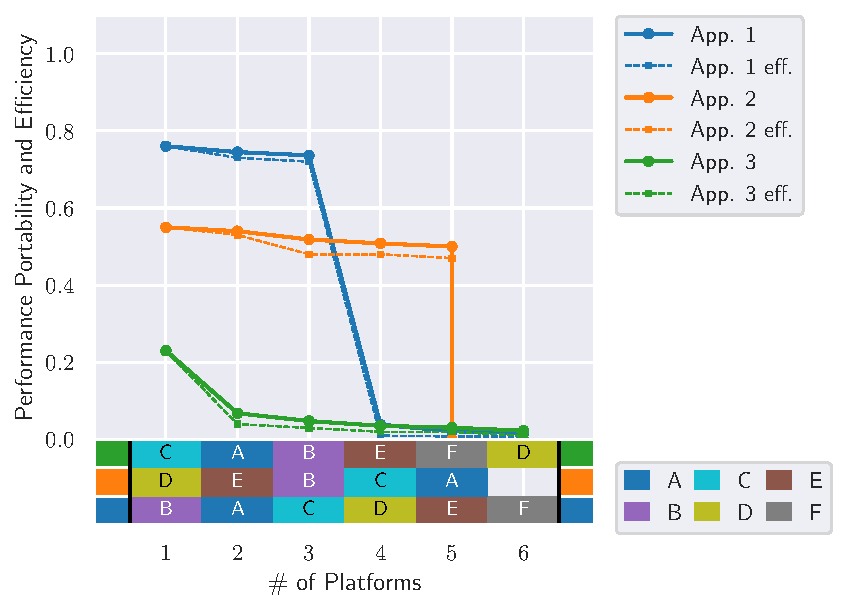
\includegraphics[width=\linewidth]{figures/02_performance_portability/example_diss_eff_cascade.pdf}
    \caption{%
    An example visualization of the architectural efficiencies of \autoref{tab:example_effs} and performance portability scores of \autoref{tab:example_pp} of the three example applications as proposed by \citet{sewall_interpreting_2020}. 
    This plot can help us to determine the set of platforms best supported by some applications. 
    }
    \label{fig:pp-example-visualization}
\end{figure}

\begin{figure}
    \centering
    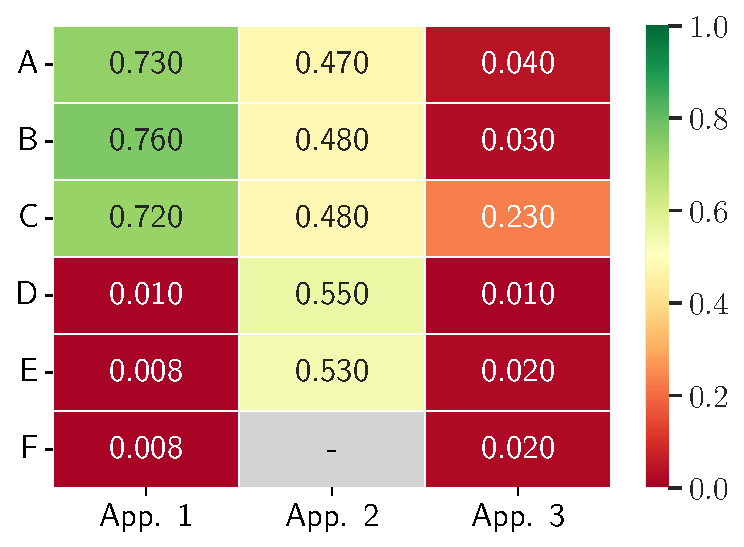
\includegraphics[width=0.75\linewidth]{figures/02_performance_portability/example_diss_eff_heat.pdf}
    \caption{%
    An example visualization of the architectural efficiencies of \autoref{tab:example_effs} as a simple heatmap makes it easy to spot the overall behavior of the three example applications. 
    }
    \label{fig:pp-example-visualization}
\end{figure}


\newpage
\cite{pennycook_navigating_2021}

\begin{itemize}
    \item it should be clear what is part of the application and what of the platform (e.g., third-party libraries)
    \item Cascade plots: \enquote{applications extending further to the right support more platforms (portability), and if they do so with higher efficiency, are more performance portable.}
    \item Productivity: subjective, approximation sufficient; they use \cite{harrell_effective_2018} code divergence with the Jaccard distance
    \item dendrogram for visualizing code divergence (by clustering)
    \item \pp-CC charts: $2D$-plane, top-right corner is the goal
    \item track performance portability and productivity as early as possible in the development process
    \begin{enumerate}
        \item identify the destination
        \item get your bearings
        \item chart the course
        \item set sail
    \end{enumerate}
\end{itemize}

\begin{definition}[Jaccard Distance SLOC~\citet{pennycook_navigating_2021}]
Given $c_i(a, p)$ as the set of source lines required to compile application $a$ and execute problem $p$ for platform $i$, the dissimilarity of the source code can be expressed as:

$$d_{i, j}(a, p) = 1 - \frac{\abs{c_i(a, p) \cap c_j(a, p)}}{\abs{c_i(a, p) \cup c_j(a, p)}}$$
\end{definition}
Here, $0$ means \enquote{single-source}, i.e., everything is shared by both platforms, and $1$ means nothing is shared. 

\begin{definition}[\pp-CC Metric~\citet{pennycook_navigating_2021}]
    $$M(a, p, H) = \min(\pp(a, p, H), CC(a, p, H))$$
\end{definition}